\documentclass[12pt]{article}
\usepackage[top=2.8cm, bottom=3cm, left=2.5cm, right=2.5cm]{geometry}
\usepackage[hidelinks]{hyperref}
\usepackage[numbers]{natbib}
\bibliographystyle{plainnat}
\usepackage{appendix}
\usepackage{caption}
\usepackage{amsmath}
\usepackage{listings}
\usepackage{setspace}
\linespread{1.2}
\lstset { %
    language=C++,
    backgroundcolor=\color{black!5}, % set backgroundcolor
    basicstyle=\ttfamily\footnotesize,% basic font setting
}
\usepackage{bchart}
\usepackage{booktabs}

\setlength{\parindent}{0em}
\setlength{\parskip}{1em}

\setlength\parindent{0pt}
\usepackage{tikz}


\title{\textbf{Parallel Computing Assignment 1 \\ Shared Memory}}

\begin{document}
\maketitle


\tableofcontents
\listoffigures
\clearpage


\section{Approach to Parallelisation}

\subsection{Introduction}

The assignment was to implement matrix relaxation for a shared memory architecture using pthreads, on a matrix $\mathcal{M}$ of variable square dimension $d$, using $t$ threads, working to a floating point precision of $p$.

My implementation uses two barriers and no other synchronisation primitives, taking advantage of the case of redundant-write data races discussed in \citep{benigndataraces} to avoid the overheads of locking a shared global variable.

\subsection{Preventing Data Races}

Data races are one of the most difficult problems arising from multithreaded code to debug, due to the seemingly random nature of how threads are scheduled \citep{highleveldataraces}. They occur when concurrent threads attempt to access a shared variable (which is not protected by an explicit synchronisation mechanism) and at least one of the accesses is a write \citep{eraser}.

I order to preserve the consistency of data being read by performing the \textit{relax} operation on a different cell, no cell can be overwritten with its new value until the new value every other cell has been calculated. This is the case regardless of whether the relaxation is performed sequentially or in parallel, and necessitates using a second matrix of the same dimensions, into which the relaxed values are written. After each complete relaxation, the two matrices can then be swapped so that the result of the most recent iteration can be relaxed, overwriting the result of the second most recent. There is of course additional space complexity associated with allocating space for $2n$ elements, but this is still linear ($\mathcal{O}(2n)$ generalises to $\mathcal{O}(n)$) and is therefore a reasonable trade-off against the overheads of alternative solutions.

Although during the process of relaxation any cell $a_{i,j}$ will be read as part of performing the \textit{relax} operation on at most four of its neighbours ($a_{i-1,j}, a_{i,j-1}, a_{i+1, j}$ and $a_{i,j+1}$), it will only ever be written to when $a_{i,j}$ itself is relaxed. This means that no synchronisation is required when writing values to the second array, as write-access to every element is guaranteed to only happen once, during which time there are no reads. Similarly, checking the precision of a cell requires one read operation in each array but no writes, so again avoids potential races.

\subsection{Division of Work}

Relaxing a square matrix of size $n \times n$ with $t$ threads requires $(n-2)^2$ cells to be relaxed each iteration, as the array boundary values remain fixed. Dividing the work as evenly as possible can be done with simple arithmetic.

All threads relax a minimum of $(n-2)^2$ div $t$ cells, where div is the integer division operation. This leaves $(n-2)^2$ mod $t$ cells remaining, and as there is no way of predicting how each thread will be scheduled and therefore which ones will finish first, for the sake of simplicity this leaves the first $((n-2)^2$ mod $t)$ threads assigned to do $((n-2)^2$ div $t) + 1$ cells each.

Calculating the precision for a given cell is not dependent on the values of any of its adjacent neighbours, so threads both relax and compute the precision for every cell they are assigned, which avoids the cost of needlessly looping again.

Since array access in C is row-major, indexing into a row's columns is a faster operation than indexing into a column's rows, so I assign cells to threads by varying the second index in the inner loop.


\subsection{Thread Work}

My approach to parallelising the solution was to reduce contention for global variables as much as possible. There are two global condition variables, \texttt{global\_continue} and \texttt{global\_done}. \texttt{global\_continue} gets set to 1 by any thread, if any of its cells did not reach the required precision, meaning another iteration is required. \texttt{global\_done} is a binary flag set only by the main thread (to 1 if the threads can return or 0 if they need to continue.)

I used two barriers to synchronise threads, as illustrated in Figures \ref{fig:workers} and \ref{fig:main}. The first is hit once all the worker threads have relaxed their assigned cells and either set \texttt{global\_continue} or not set it. Once the main thread hits also this barrier, the worker threads hit the second barrier and wait. The main thread resets \texttt{global\_continue} if it has been set, ready for the next iteration. If \texttt{global\_continue} was zero, all threads have finished, so the main thread sets \texttt{global\_done} which will cause all the threads to return.

There is obvious contention for \texttt{global\_continue} between all threads which may want to increment it. However, I avoided having to use a lock by treating any non-zero value as \texttt{true}. Either an arbitrary number of threads assign \texttt{global\_continue = 1} in succession (which will be read by the main thread as \texttt{true}) or two or more of the assignments happen simultaneously and the value is still a non-zero one (and will therefore still be read by the main thread as \texttt{true}.) This particular case of race has been found to be acceptably safe \citep{benigndataraces}.

\begin{figure}[!htb]
    \begin{minipage}{.47\textwidth}
        \hspace{-1.6cm}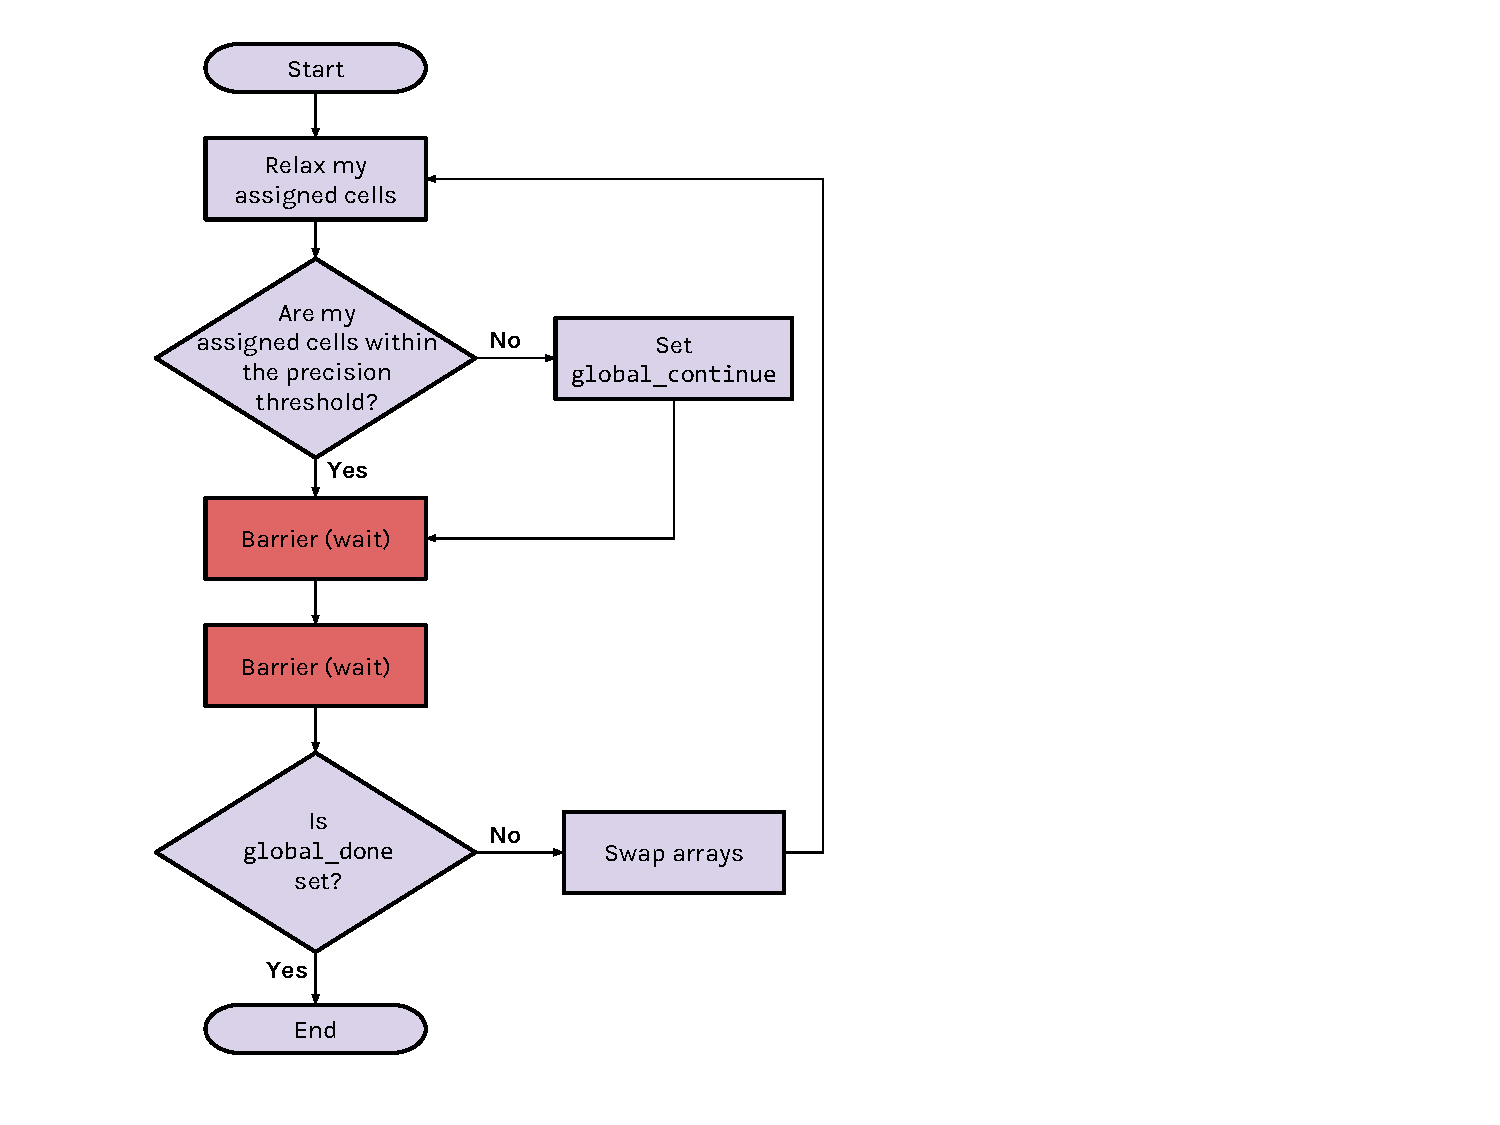
\includegraphics[width=2.4\textwidth]{img/workersflowchart.pdf}
        \caption{Worker thread control flow}
        \label{fig:workers}
    \end{minipage}\hspace{1.65cm}
    \begin{minipage}{0.47\textwidth}
       \hspace{-1cm}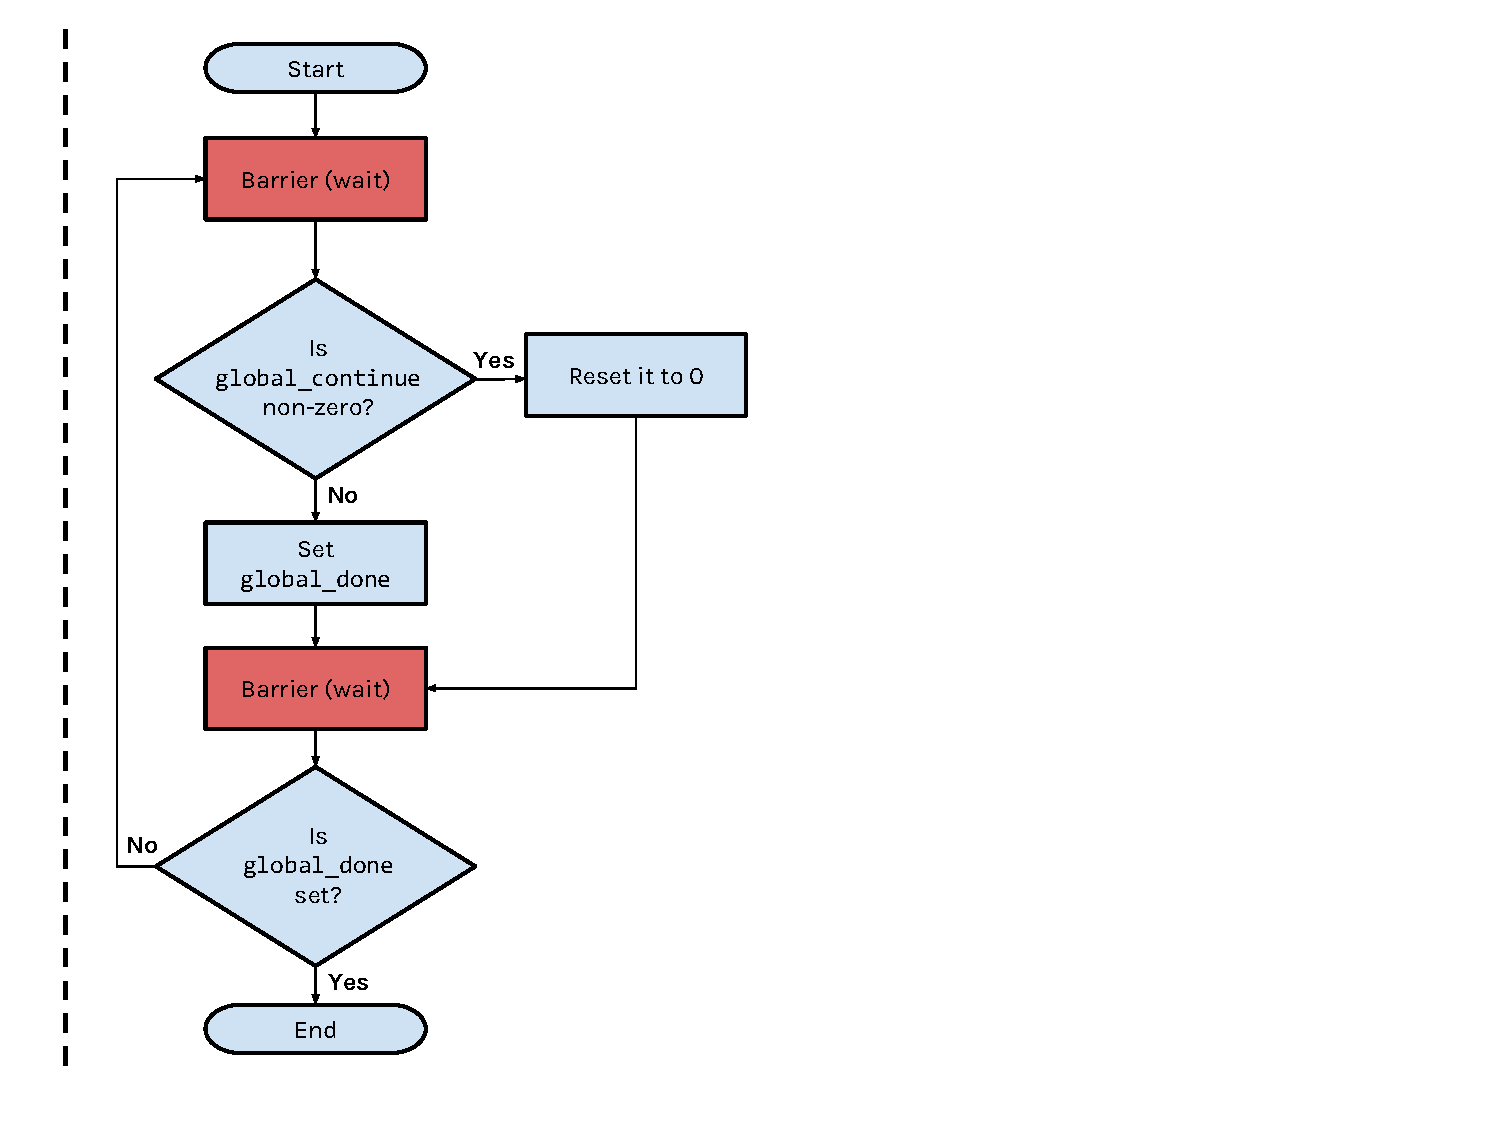
\includegraphics[width=2.4\textwidth]{img/mainflowchart.pdf}
        \caption{Main thread control flow}
        \label{fig:main}
    \end{minipage}
\end{figure}
None of my worker threads allocate thread-local variables on the heap, as this is unnecessary and also requires allocator and deallocator synchronisation across every thread \citep{contention}.

\section{Correctness Testing}

To verify that my implementation of relaxation was correct, I manually calculated every step in relaxing a matrix and verified not only that both solutions terminated after the same number of iterations, but also that after each iteration, my matrix was identical to the computed one. Both my hand-computed relaxation (below) and my single-threaded implementation required four iterations to relax the 5$\times$5 matrix to a precision of 0.75.
\hspace{-0.2cm}\begin{minipage}{.5\textwidth}
$$
\begin{matrix}
1.000000 & 1.000000 & 1.000000 & 1.000000 & 1.000000 \\
1.000000 & 3.000000 & 7.000000 & 2.000000 & 1.000000 \\
1.000000 & 8.000000 & 6.000000 & 5.000000 & 1.000000 \\
1.000000 & 9.000000 & 0.000000 & 4.000000 & 1.000000 \\
1.000000 & 1.000000 & 1.000000 & 1.000000 & 1.000000 \\
\end{matrix}
$$
$$
\begin{matrix}
1.000000 & 1.000000 & 1.000000 & 1.000000 & 1.000000 \\
1.000000 & 4.250000 & 3.000000 & 3.500000 & 1.000000 \\
1.000000 & 4.750000 & 5.000000 & 3.250000 & 1.000000 \\
1.000000 & 2.500000 & 5.000000 & 1.750000 & 1.000000 \\
1.000000 & 1.000000 & 1.000000 & 1.000000 & 1.000000 \\
\end{matrix}
$$
$$
\begin{matrix}
1.000000 & 1.000000 & 1.000000 & 1.000000 & 1.000000 \\ 
1.000000 & 2.437500 & 3.437500 & 2.062500 & 1.000000 \\ 
1.000000 & 3.187500 & 4.000000 & 2.812500 & 1.000000 \\ 
1.000000 & 2.937500 & 2.562500 & 2.562500 & 1.000000 \\ 
1.000000 & 1.000000 & 1.000000 & 1.000000 & 1.000000 \\ 
\end{matrix}
$$
$$
\begin{matrix}
1.000000 & 1.000000 & 1.000000 & 1.000000 & 1.000000 \\ 
1.000000 & 2.156250 & 2.375000 & 2.062500 & 1.000000 \\ 
1.000000 & 2.593750 & 3.000000 & 2.406250 & 1.000000 \\ 
1.000000 & 1.937500 & 2.625000 & 1.843750 & 1.000000 \\ 
1.000000 & 1.000000 & 1.000000 & 1.000000 & 1.000000 \\ 
\end{matrix}
$$
$$
\begin{matrix}
1.000000 & 1.000000 & 1.000000 & 1.000000 & 1.000000 \\ 
1.000000 & 1.742188 & 2.054688 & 1.695312 & 1.000000 \\ 
1.000000 & 2.023438 & 2.500000 & 1.976562 & 1.000000 \\ 
1.000000 & 1.804688 & 1.945312 & 1.757812 & 1.000000 \\ 
1.000000 & 1.000000 & 1.000000 & 1.000000 & 1.000000 \\
\end{matrix}
$$
\end{minipage}\hspace{1.5cm}
\begin{minipage}{.5\textwidth}
\vspace{0.6cm}
	\textbf{Initial Matrix}\\[1.9cm]
	Max $\Delta$: $abs$(9-2.5) = 6.5\\
	6.5 $\geq$ 0.75 so continue.\\[1.6cm]
	
	Max $\Delta$: $abs$(5-2.5625) = 2.4375\\
	2.4375 $\geq$ 0.75 so continue.\\[1.6cm]
	
	Max $\Delta$: $abs$(3.4375-2.375) = 1.0625\\
	1.0625 $\geq$ 0.75 so continue.\\[1.6cm]
	
	Max $\Delta$: $abs$(2.625-1.9453125) = 0.6796875\\
	0.6796875 $<$ 0.75 (done).\\[1.9cm]
	\textbf{Relaxed matrix (after 4 iterations)}
\end{minipage}

The hand-computed results show my checking of the maximum delta for each array after relaxing it to determine whether another iteration is required. Once I verified that my implementation was correct with one thread, I relaxed under the same conditions with 2-9 threads, printing all intermediate values and the iteration count at termination. I then used the Unix \texttt{diff} utility to check all 9 outputs were identical. These files have been included in the \texttt{correctness} directory, for verification.

\section{Scalability Investigation}
\subsection{Fixed Problem Size}
Once I had verified the correctness of my relaxation implementation, I chose a fixed array size and precision, and ran my program relaxing the same array with 1-16 threads. The time, speedup and efficiency (speedup achieved by $n$ processors divided by $n$ \citep{speedup}) for this can be seen in Figures \ref{fig:basict} and \ref{fig:basics}. 
\begin{figure}[!htb]
    \begin{minipage}{.46\textwidth}
        \hspace{-0.8cm}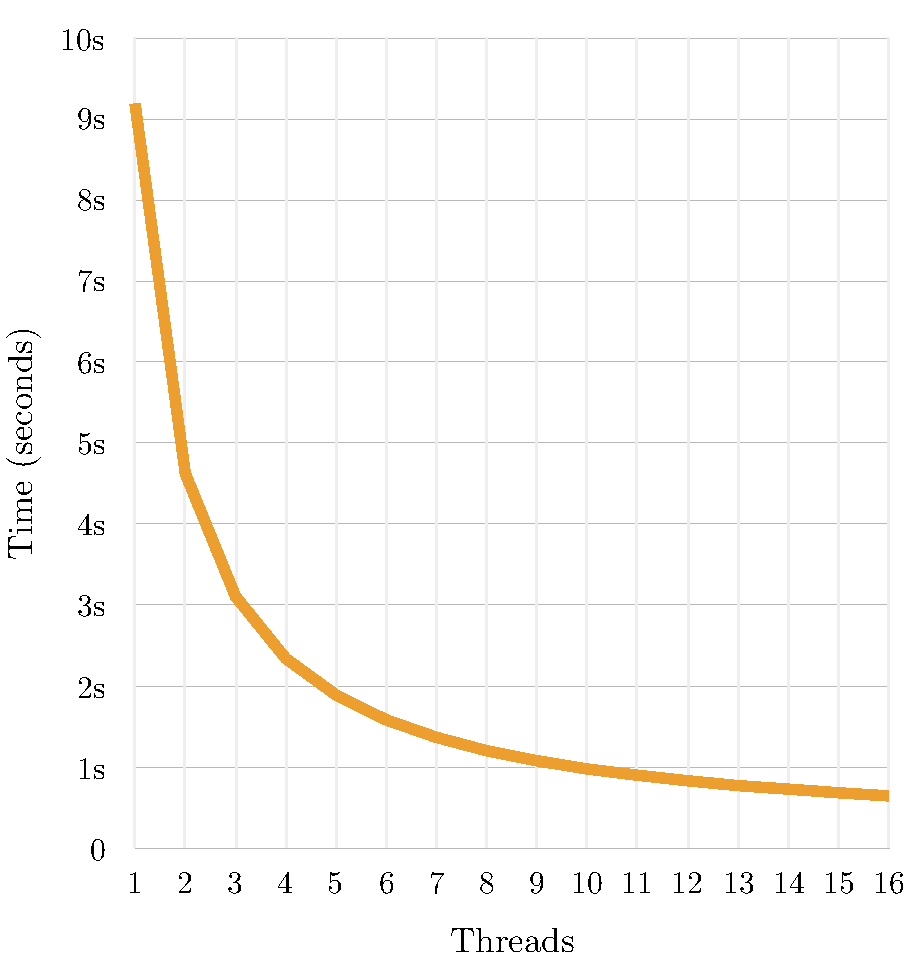
\includegraphics[width=1.1\textwidth]{img/basic-threads-time.pdf}
        \centering\caption{Time for 1-16 threads to relax the same matrix, $d=1000$, $p=0.5$}
        \label{fig:basict}
    \end{minipage}\hspace{0.4cm}
    \begin{minipage}{0.53\textwidth}
       \hspace{-0.8cm}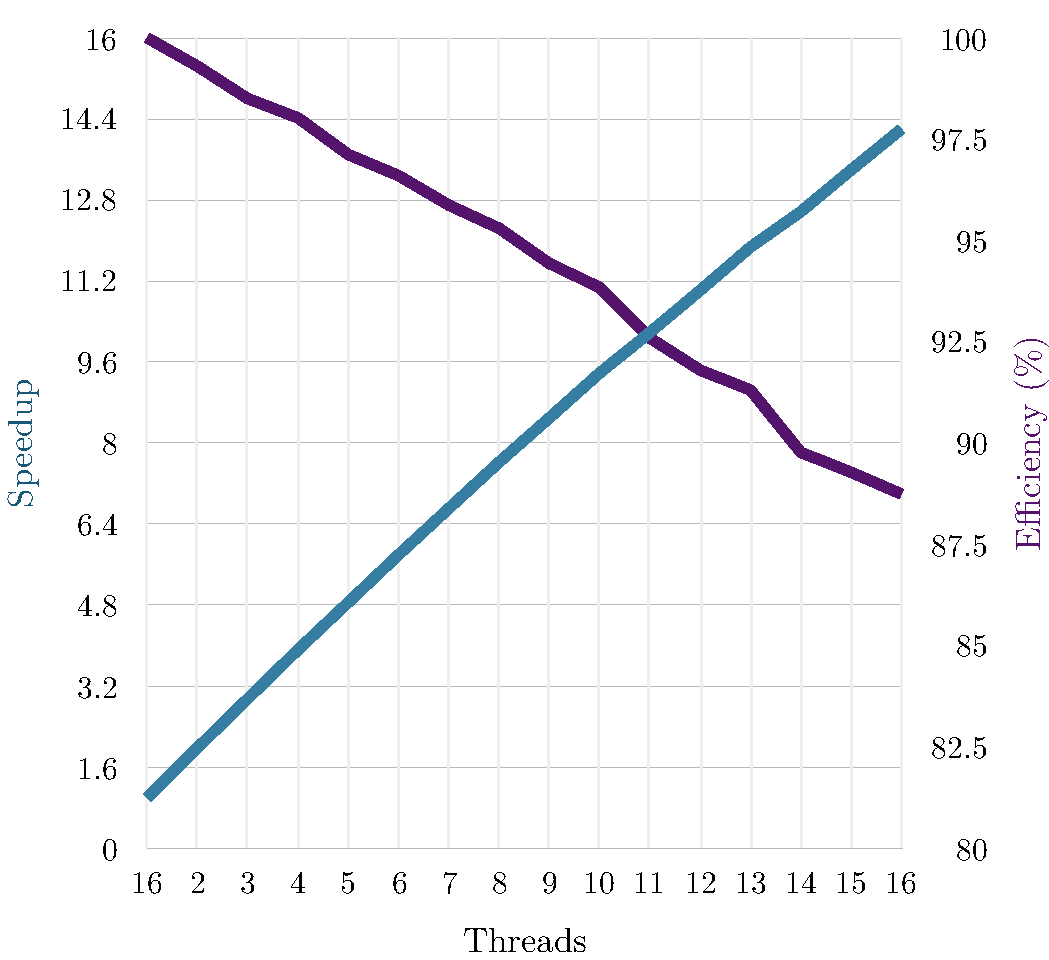
\includegraphics[width=1.1\textwidth]{img/basic-threads-speedup.pdf}
        \centering\caption{Speedup and efficiency achieved by 1-16 threads relaxing the matrix, $d=1000$, $p=0.5$}
        \label{fig:basics}
    \end{minipage}
\end{figure}

Each thread\footnote{The thread counts specified in this section refer to worker threads, i.e. the main thread is not included.} saw efficiency reduce, as the speedup had a progressively smaller impact on the time reduction (diminishing returns; \citep{Amdahl}). This is consistent with Amdahl's law, a corollary of which states that for P processors and a computation whose sequential proportion is denoted $f$, predicted speedup is bound by $\frac{1}{f}$ \citep{springer}. Working backwards from this upper bound and assuming a maximum speedup of 14.5, this would imply that the sequential proportion of my solution is $\leq 0.069$, or 6.9\% of the total computation for this fixed problem size. It is important to note that the sequential proportion is not fixed, as changing the number of threads, precision or dimensions would alter the overhead needed to allocate, assign thread work, and wait at barriers.

The speedup I achieved for this problem size was sub-linear, but close to linear. The sequential proportion of the computation appears to become the limiting factor above 16 threads, preventing further speedup through parallelisation.\footnote{Full data in Appendix \ref{sec:basic}.} In order to verify this, I repeated the experiment with even numbers of threads between 2 and 32 on the same matrix. The resulting time, speedup and efficiency values can be seen in Figures \ref{fig:clifft} and \ref{fig:cliffs}, with the values for 1 thread (i.e. the sequential computation) left in for comparison.\footnote{Full data in Appendix \ref{sec:cliff}.}

\begin{figure}[!htb]
    \begin{minipage}{.46\textwidth}
        \hspace{-0.8cm}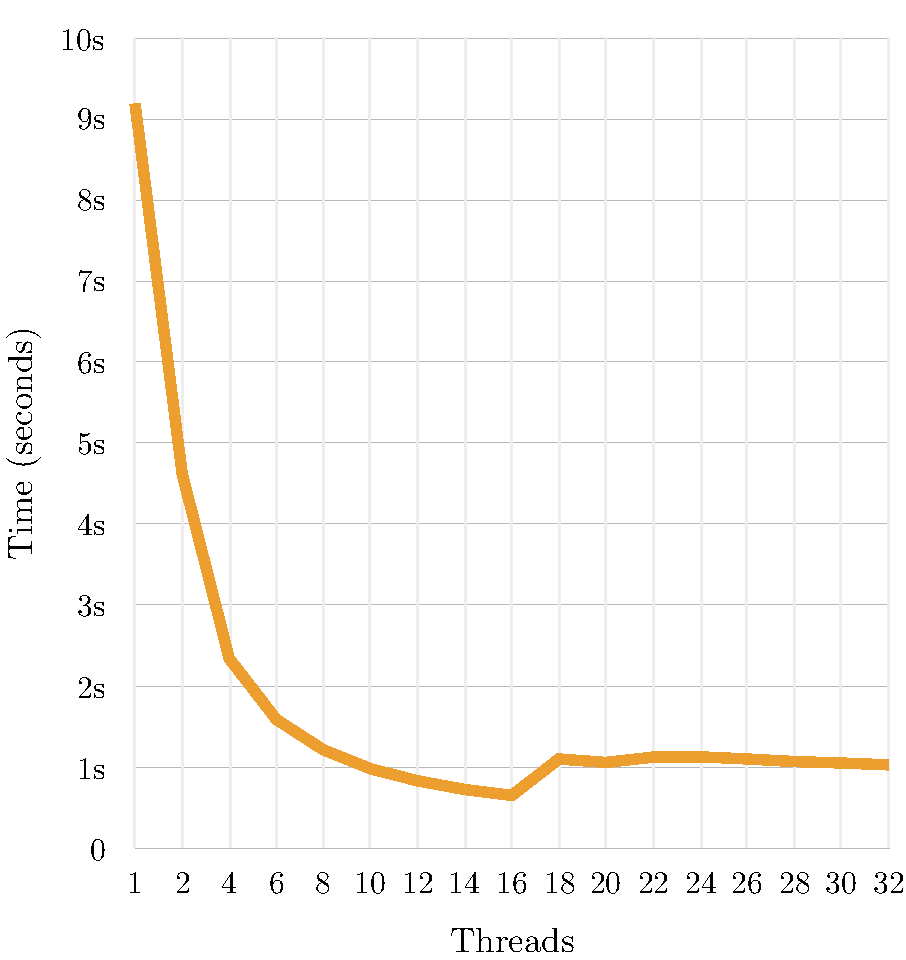
\includegraphics[width=1.1\textwidth]{img/cliff-threads-time.pdf}
        \centering\caption{Time for 2-32 threads to relax the same matrix, $d=1000$, $p=0.5$}
        \label{fig:clifft}
    \end{minipage}\hspace{0.4cm}
    \begin{minipage}{0.53\textwidth}
       \hspace{-0.8cm}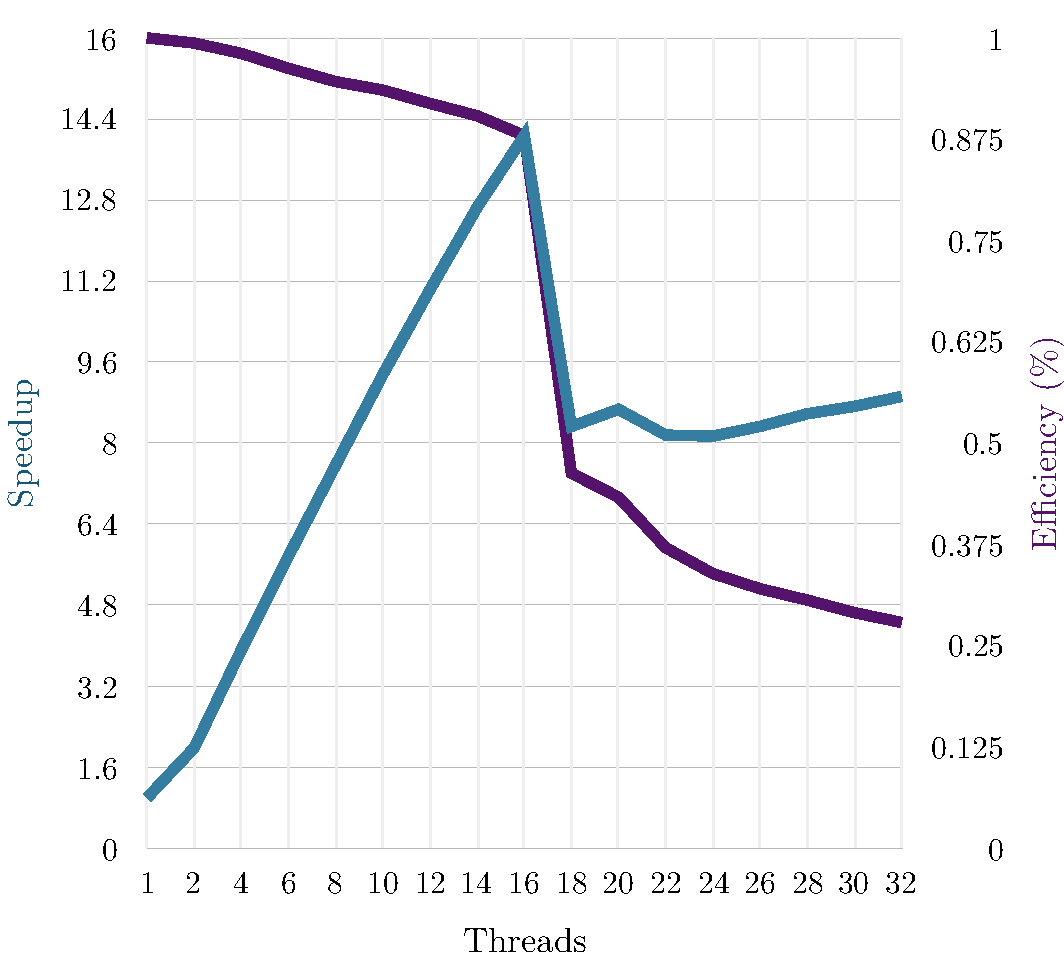
\includegraphics[width=1.1\textwidth]{img/cliff-threads-speedup.pdf}
        \centering\caption{Speedup achieved by 2-32 threads relaxing the matrix, $d=1000$, $p=0.5$}
        \label{fig:cliffs}
    \end{minipage}
\end{figure}

\subsection{Variable Problem Size}

The second factor I tested was the effect of varying the matrix dimensions on the time, for various thread counts. The results of this can be seen in Figure \ref{fig:dimension}\footnote{Full data in Appendix \ref{sec:dt}}. The x-axis in the graph is scaled with respect to dimensions but not size, since the actual computation required for each dimension is proportional to the square of the dimension, not the dimension itself.

\begin{figure}[h!]
	\centering
	\hspace{-0.5cm}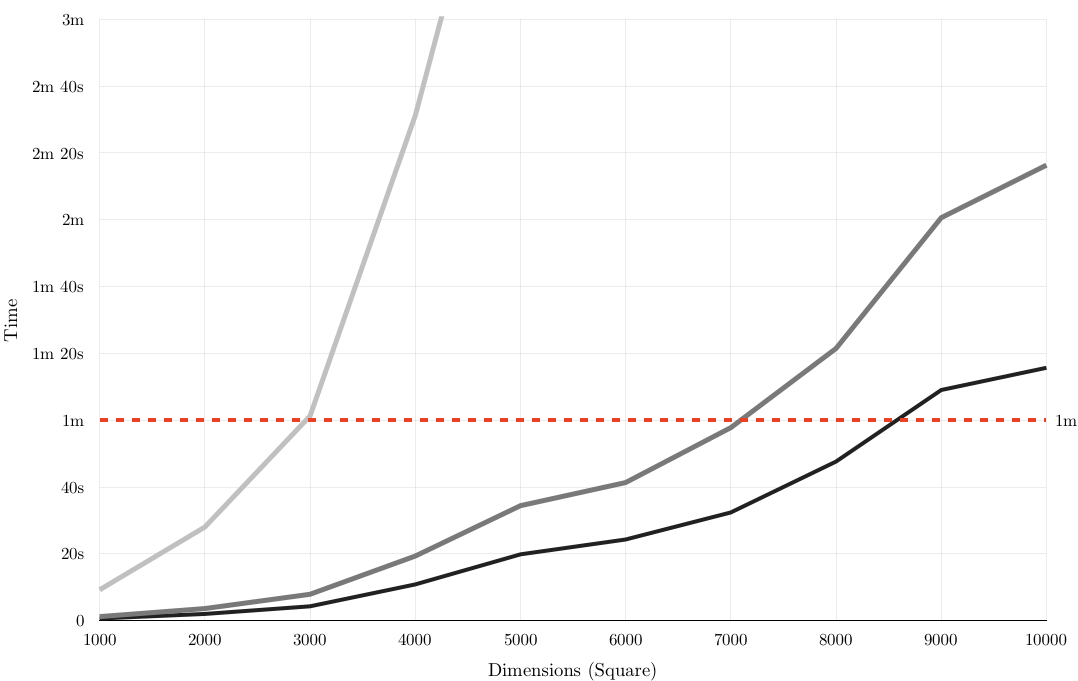
\includegraphics[width=.85\textwidth]{img/dimension-time}
	\caption{Matrix dimensions against time for 1 (light grey), 8 (medium grey) and 16 (dark grey) threads.}
	\label{fig:dimension}
\end{figure}

Consider the values which intersect the dotted line in Figure \ref{fig:dimension}. In one minute, one thread can relax a 3000$^2$ matrix, with 9,000,000 elements. In the same amount of time, eight threads can relax a 7000$^2$ matrix (49,000,000 elements, and a speedup of 7) and sixteen threads can relax approximately 8500$^2$ (72,250,000 elements, and a speedup of 8.03). The relative drop in speedup from 1-8 and 8-16 threads again demonstrates the effect  of diminishing returns and efficiency; the efficiency of eight threads is $7\div{}8=$ 87.5\%; for sixteen threads this becomes $8.03\div{}16=$ 50.1\%. It is important to note however that the most efficient number of processors is not the number which will yield the greatest absolute speedup. Mathematically, peak efficiency is reached by maximising $\frac{\text{speedup}}{n}$, which is equivalent to $\frac{T_\text{seq}}{n\times{T_n}}$. $T_\text{seq}$ is fixed, so maximum efficiency is found minimising $n\times{T_n}$; the solution to which will be $n=1$ unless speedup is superlinear. 

\subsection{Precision}

I conducted a single experiment into the effects of lowering the precision threshold on the time and iterations required for my solution to terminate. Below are the results for a fixed array with $d=500$ and 16 threads\footnote{Full data in Appendix \ref{sec:prec}}, showing iterations and time increasing at the same rate as the precision threshold is lowered.

\begin{figure}[h!]
	\hspace{-0.8cm}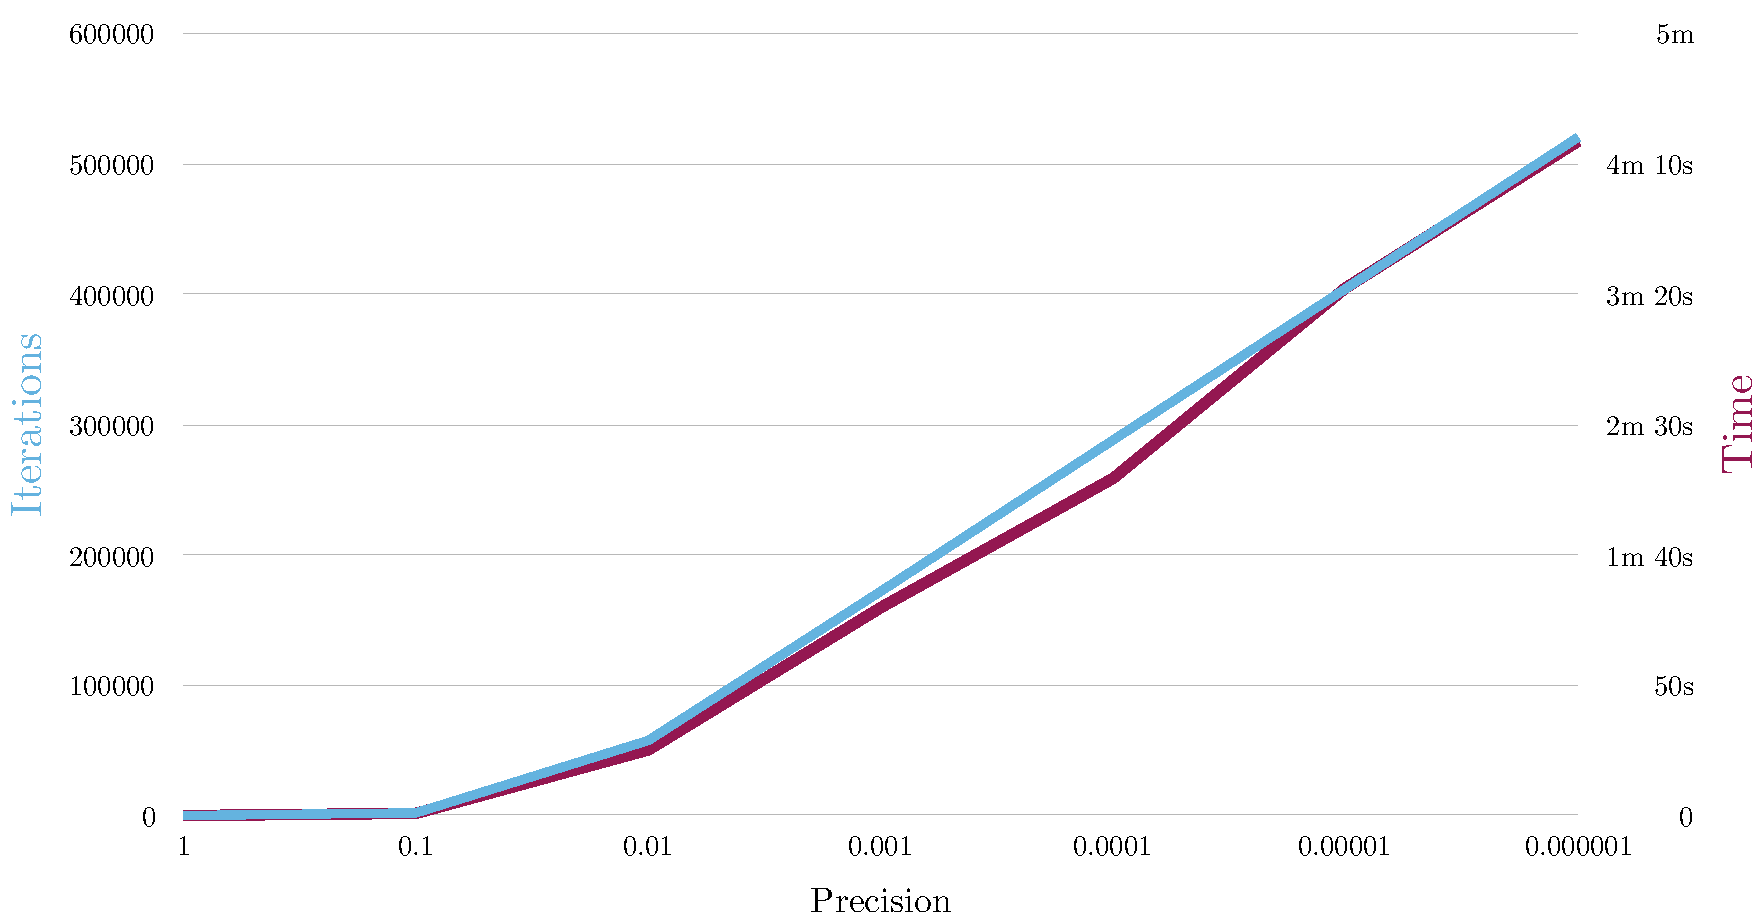
\includegraphics[width=1.1\textwidth]{img/prec-time.pdf}
	\caption{Precision values against iterations and time}
	\label{fig:precision}
\end{figure}
I tried to run my solution on a precision of 0.0000001, but it timed out on Balena, due to either exceeding the 15 minute limit while relaxing, or reaching the point at which applying the relax operation left every cell unchanged. Not every matrix when relaxed to under a given precision will terminate. My implementation does not attempt to identify these cases and would therefore loop infinitely for precision values which aren't reachable for a given matrix.

\section{Cycle Accounting}

To determine whether there were any simple optimisations I could make to my implementation to improve speeds, I ran it on Balena under Valgrind, using the \texttt{callgrind} and \texttt{cachegrind} tools. I then exported the output file and analysed it with qcachegrind\footnote{https://kcachegrind.github.io/html/Home.html}.

In \texttt{callgrind}, I ordered functions by cycle count (ignoring cycle counts of their callees). Although cycle count is not perfectly analogous to latency, it is the closest metric callgrind provides. This allowed me to see the functions which were dominating execution cycles, as shown in Figure \ref{fig:top-cycles}.
\begin{figure}[!h]
\centering
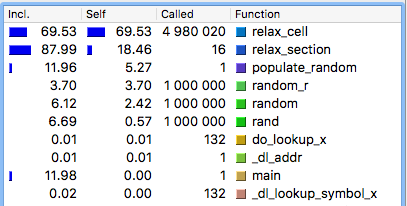
\includegraphics[width=.5\textwidth]{img/top-ten.png}
\caption{The top ten functions by self-cycles}
\label{fig:top-cycles}
\end{figure}
At the lower end of the list are functions which can be expected such as \texttt{main}, functions prefixed \texttt{dl\_} which are the dynamic linker loading pthread library functions, and functions responsible for populating the array with random numbers. None of these are associated with the actual relaxation logic. 

\begin{figure}[htbp!]
\hspace{-0.7cm}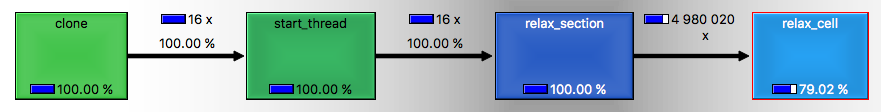
\includegraphics[width=1.1\textwidth]{img/cg.png}
\caption{Call graph showing \texttt{relax\_cell} and \texttt{relax\_section}}
\label{fig:cg}
\end{figure}

The top two functions; \texttt{relax\_cell} and its caller, my thread function \texttt{relax\_section} account for the vast majority of cycles. Figure \ref{fig:cg} shows that the 4,980,020 calls (over 5 iterations) to \texttt{relax\_cell} account for 79.02\% of the cycles accross the 16 (one for each thread) calls to  \texttt{relax\_section}.

There was no obvious improvement which could be made to the logic in \texttt{relax\_cell}, as Figure \ref{fig:source-cycles} shows the average cycles to be fairly similar for all source lines which need to access the array (implying the cycles are due to load latency of the data), and for the assignment of the variable \texttt{new} (where the cycles would be due to latency of the store).

To confirm this, I used the \texttt{cachegrind} tool on the same input and looked at the L1 misses for reads and writes in \texttt{relax\_cell} (See Figure \ref{fig:source-misses}.)

\begin{figure}[htbp!]
    \begin{minipage}{.49\textwidth}
        \hspace{-0.3cm}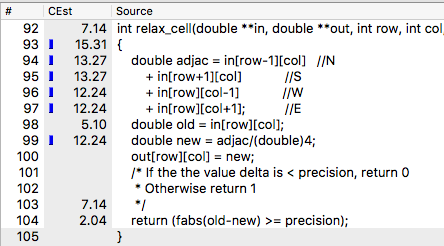
\includegraphics[width=\textwidth]{img/source-cycles}
        \centering\caption{Cycles detection averages in \texttt{relax\_cell}}
        \label{fig:source-cycles}
    \end{minipage}\hspace{0.8cm}
    \begin{minipage}{0.49\textwidth}
       \hspace{-0.3cm}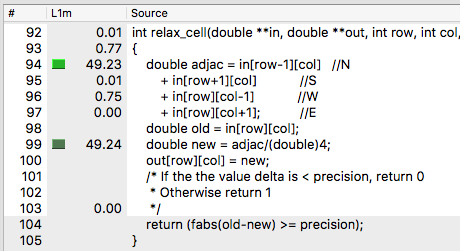
\includegraphics[width=\textwidth]{img/source-misses.png}
        \centering\caption{L1 Cache Read (light green) and Write (dark green) misses in \texttt{relax\_cell}}
        \label{fig:source-misses}
    \end{minipage}
\end{figure}

There is no easy fix for cache misses, as this is clearly a physical constraint and therefore machine-specific. Consequentially, as I had identified \texttt{relax\_cell} as the single critical performance hotspot in my application, I did not do any further performance tuning as it would have yielded inconsequential improvements.

I have included the output from valgrind in both \texttt{callgrind} and \texttt{cachegrind} mode in the \texttt{valgrind} directory, from which all of the figures in this section can be reconstructed and explored. The options used for this run of my program were $d=1000$, $p=5.0$ and $t=16$.


\clearpage


\bibliography{references}

\begin{appendices}

\clearpage
\section{Full Testing Results}
\subsection{Time and Speedup for 1-16 threads, $d=1000$, $p=0.5$}
\footnotesize{\label{sec:basic}
\begin{center}
\begin{tabular}{|l|l|l|}
\hline
Threads	& Time & Speedup  \\
\hline
1 & 9s 187ms & 1 \\
2 & 4s 626ms & 1.986 \\
3 & 3s 109ms & 2.955 \\
4 & 2s 343ms & 3.921 \\
5 & 1s 892ms & 4.856 \\
6 & 1s 585ms & 5.796 \\
7 & 1s 369ms & 6.711 \\
8 & 1s 205ms & 7.624 \\
9 & 1s 81ms & 8.499 \\
10 & 979ms & 9.384 \\
11 & 902ms & 10.185 \\
12 & 834ms & 11.016 \\
13 & 774ms & 11.87 \\
14 & 731ms & 12.568 \\
15 & 686ms & 13.392 \\
16 & 647ms & 14.199 \\
\hline
\end{tabular}
\end{center}}

\subsection{Time and Speedup for 2-32 threads, $d=1000$, $p=0.5$}
\footnotesize{\label{sec:cliff}
\begin{center}
\begin{tabular}{|l|l|l|}
\hline
Threads	& Time & Speedup  \\
\hline
2 & 4s 624ms & 1.987 \\
4 & 2s 342ms & 3.923 \\
6 & 1s 591ms & 5.774 \\
8 & 1s 214ms & 7.568 \\
10 & 982ms & 9.355 \\
12 & 833ms & 11.029 \\
14 & 726ms & 12.654 \\
16 & 653ms & 14.069 \\
18 & 1s 103ms & 8.329 \\
20 & 1s 60ms & 8.667 \\
22 & 1s 126ms & 8.159 \\
24 & 1s 129ms & 8.137 \\
26 & 1s 103ms & 8.329 \\
28 & 1s 71ms & 8.578 \\
30 & 1s 53ms & 8.725 \\
32 & 1s 30ms & 8.919 \\
\hline
\end{tabular}
\end{center}}

\subsection{Dimensions against time, $p=0.5$, $t=\{1, 8, 16\}$}
\footnotesize{\label{sec:dt}
\begin{center}
\begin{tabular}{|l|l|l|l|}
\hline
Dimension & 1 Thread & 8 Threads & 16 Threads \\
\hline
1000 & 9s 231ms & 1s 207ms & 646ms \\
2000 & 28s 13ms & 3s 616ms & 2s 7ms \\
3000 & 1m 1s 257ms & 7s 896ms & 4s 291ms \\
4000 & 2m 31s 143ms & 19s 331ms & 10s 843ms \\
5000 & 4m 29s 167ms & 34s 413ms & 19s 845ms \\
6000 & 5m 23s 100ms & 41s 339ms & 24s 290ms \\
7000 & 7m 29s 558ms & 57s 778ms & 32s 389ms \\
8000 & (timed out) & 1m 21s 480ms & 47s 624ms \\
9000 & (timed out) & 2m 0s 608ms & 1m 9s 36ms \\
10000 & (timed out) & 2m 16s 340ms & 1m 15s 692ms \\
\hline
\end{tabular}
\end{center}}

\subsection{Precision against iterations and time, $d=500$, $t=16$}
\footnotesize{\label{sec:prec}
\begin{center}
\begin{tabular}{|l|l|l|}
\hline
Precision	& Time & Iterations  \\
\hline
1 & 38ms & 78 \\
0.1 & 872ms & 2160 \\
0.01 & 25s 239ms & 57755 \\
0.001 & 1m 19s 879ms & 172235 \\
0.0001 & 2m 9s 480ms & 288416 \\
0.00001 & 3m 22s 586ms & 404599 \\
0.000001 & 4m 18s 886ms & 520783 \\
0.0000001 & (timed out) & (timed out) \\
\hline
\end{tabular}
\end{center}}

	
\end{appendices}

\end{document}